
\subsubsection{01.11.14}

\begin{enumerate}
	\item Время начала и окончания собрания:
	16:00 – 21:40
	\item Цели собрания:
	\begin{enumerate}
	  \item Закрепить отвалившееся на предыдущем занятии ребро жесткости.
	  
	  \item	Установить 2 оставшиеся перекладины на подъемник.
	  
	  \item	Закрепить ремень на подъемнике.
	  
	  \item	Испытать подъемник.
	  
    \end{enumerate}
    
	\item Проделанная работа:
	\begin{enumerate}
	  \item	Ребро жесткости было решено закрепить не на термоклей, поскольку такое крепление недостаточно прочно, а на болты. В связи с этим его пришлось закрепить выше остальных ребер для того, чтобы шляпки болтов не мешали движению подъемника.
      
      \item Две оставшиеся перекладины были закреплены в отверстиях, просверленных ранее, и зафиксированы термоклеем.
      
      \item	Для испытания подъемника в действии, на нем был закреплен ремень. На данный момент он был закреплен узлом, однако для окончательной версии его будет необходимо зафиксировать иначе: сделать петлю, которая будет держаться за последнюю перекладину и прошить ее с помощью ниток.
      
      \begin{figure}[H]
      	\begin{minipage}[h]{1\linewidth}
      		\center{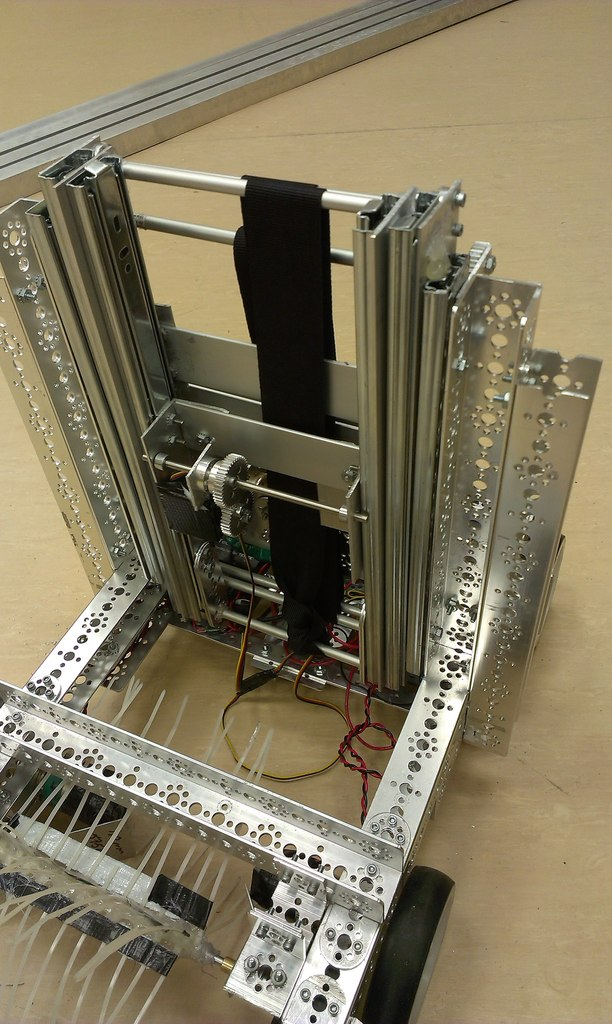
\includegraphics[scale=0.25]{days/images/9lyRPcwuEBA}}
      		\caption{Подъемник завершен}
      	\end{minipage}
      \end{figure}
      
      \item	При испытании подъемника путем вытягивания ремня руками, было выяснено, что раздвигание подъемника требует некоторых усилий, с которыми 2 привода должны справиться. Складывание подъемника проходило сложнее, поскольку внутренняя пара реек не опускалась под действием своего веса. Было решено, что если после установки на эту пару реек ковша она все равно не будет опускаться, мы дополнительно утяжелим ее. Кроме того, мы надеялись решить проблемы со складыванием подъемника, уменьшив трение ремня об перекладину. К сожалению, нами пока не было найдено подходящей детали для осуществления этого замысла.
      
      \item	На робота были установлены приводы для раздвигания подъемника (далее механизм раздвигания подъемника будет называться лебедкой).
      
      \item	Из-за того, что подъемник опускался внутрь робота, под ним не осталось места для NXT-блока, и его было необходимо переместить в другое место. Куда переместить NXT-блок, решено пока не было.
      
      \begin{figure}[H]
      	\begin{minipage}[h]{1\linewidth}
      		\center{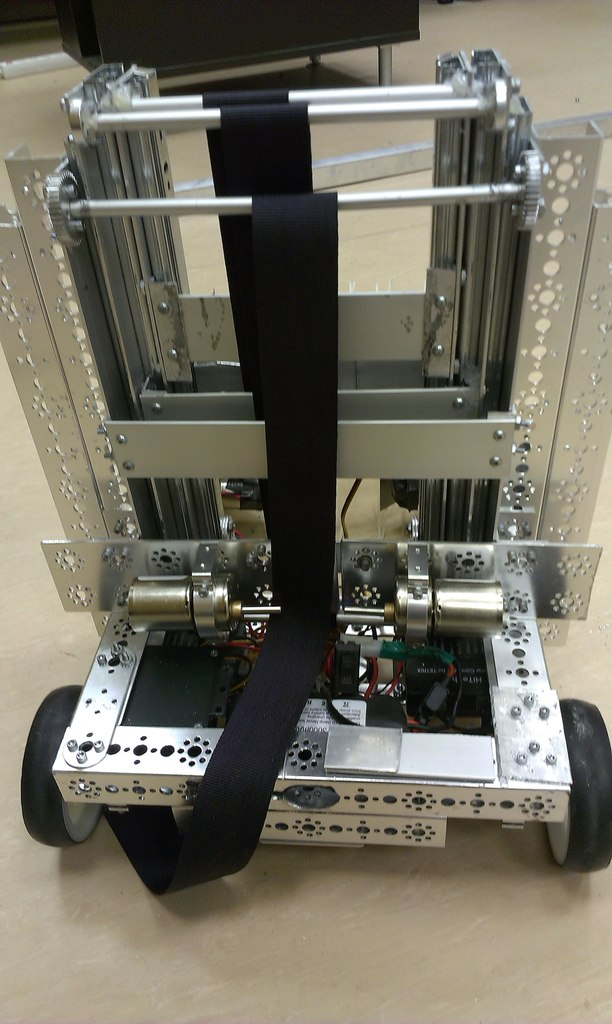
\includegraphics[scale=0.25]{days/images/-E1JUAJCMPw}}
      		\caption{Приводы для раздвигания подъемника}
      	\end{minipage}
      \end{figure}
      
    \end{enumerate}
    
	\item Итоги собрания: 
	\begin{enumerate}
	  \item	Ребро жесткости установлено.
	  
	  \item	Механизм подъемника завершен.
	  
	  \item	Подъемник испытан в тестовом режиме.
	  
	  \item	Начата установка механизма лебедки.
	  
    \end{enumerate}
    
	\item Задачи для последующих собраний:
	\begin{enumerate}
	  \item	Завершить работу над механизмом лебедки.
	  
	  \item	Установить драйвер приводов для лебедки.
	  
	  \item	Закрепить ремень с помощью ниток.
	  
	  \item	Переместить NXT-блок на новое место.
	  
    \end{enumerate}     
\end{enumerate}
\fillpage
